\section{\freest{} is for programming}
\label{sec:programming}

\freest{} is a basic implementation of the language introduced by
Thiemann and Vasconcelos~\cite{DBLP:conf/icfp/ThiemannV16}.
%
We have chosen the concrete syntax to be aligned with that of Haskell,
as much as possible. A \freest{} program is a collection of type
abbreviations, datatype and function (or value) declarations. Function
\lstinline|main| runs the program.

Our example serializes a tree object on a channel. The aim is to
transform a tree by interacting with a remote server. The client
process streams a tree on a (single) channel. In addition, for each
node sent, an integer is received. The server process reads a tree
from the other end of the channel and, for each node received, sends
back the sum of the integer values under (and including) that
node.
%
\newcommand{\leaf}{$\bullet$}
%
As an example, our program transforms the tree on the left into the one
on the right, where we use \leaf{} to abbreviate \lstinline|Leaf|.

\begin{center}
  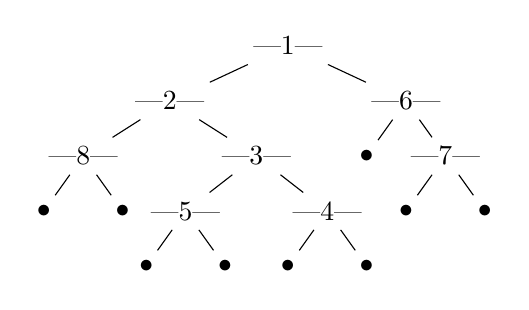
\begin{tikzpicture}[level 1/.style={sibling distance=3cm}, level
    2/.style={sibling distance=2.2cm}, level 3/.style={sibling
      distance=1.8cm}, level 4/.style={sibling distance=1cm}, level
    distance = 7mm]
    \node{\lstinline|1|} child { node {\lstinline|2|} child [level
      3/.append style={sibling distance=1cm}]{ node {\lstinline|8|}
        child { node {\leaf}} child { node {\leaf}}} child { node
        {\lstinline|3|} child { node {\lstinline|5|} child { node
            {\leaf}} child { node {\leaf}}} child { node
          {\lstinline|4|} child { node {\leaf}} child { node {\leaf}}
        }}} child[level 2/.append style={sibling distance=1cm}] { node
      {\lstinline|6|} child { node {\leaf}} child[level 3/.append
      style={sibling distance=1cm}] { node {\lstinline|7|} child {
          node {\leaf}} child { node {\leaf}}}} ;
  \end{tikzpicture}
  \hspace*{2em}
  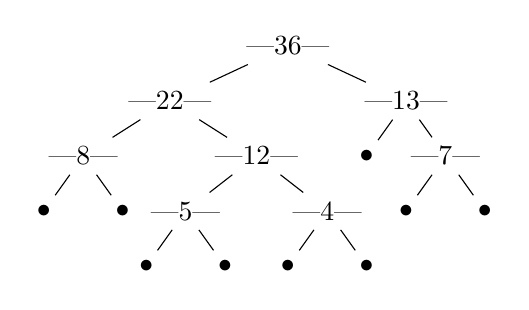
\begin{tikzpicture}[level 1/.style={sibling distance=3cm}, level
    2/.style={sibling distance=2.2cm}, level 3/.style={sibling
      distance=1.8cm}, level 4/.style={sibling distance=1cm}, level
    distance = 7mm]
    \node{\lstinline|36|} child { node {\lstinline|22|} child [level
      3/.append style={sibling distance=1cm}]{ node {\lstinline|8|}
        child { node {\leaf}} child { node {\leaf}}} child { node
        {\lstinline|12|} child { node {\lstinline|5|} child { node
            {\leaf}} child { node {\leaf}}} child { node
          {\lstinline|4|} child { node {\leaf}} child { node {\leaf}}
        }}} child[level 2/.append style={sibling distance=1cm}] { node
      {\lstinline|13|} child { node {\leaf}} child[level 3/.append
      style={sibling distance=1cm}] { node {\lstinline|7|} child {
          node {\leaf}} child { node {\leaf}}}} ;
  \end{tikzpicture}
\end{center}

% The datatype for trees, \lstinline|Tree|, was introduced before.  
We need a channel capable of transmitting a tree. The type below
describes a variant of the \lstinline|TreeChannel| introduced in the
previous section that not only sends a tree, but, for each
\lstinline|Node|, also receives back an integer value.
%
\begin{lstlisting}
type TreeC = +{Leaf: Skip, Node: !Int;TreeC;TreeC;?Int}
\end{lstlisting}

The \lstinline|+| type constructor introduces an internal choice (the
process in possession of the channel end chooses) with two
alternatives, labelled \lstinline|Leaf| and \lstinline|Node|. These
two labels should not be confused with the constructors of datatype
\lstinline|Tree|. The \lstinline|Leaf| branch states that no further
interaction is possible on the channel (denoted by \lstinline|Skip|);
the \lstinline|Node| branch writes an integer value, followed by two
trees, and terminates by reading an integer value
(\lstinline|!Int;TreeC;TreeC;?Int|).
%
The type declaration introduces an \emph{abbreviation} to a recursive
type \lstinline|rec x. +{Leaf: Skip, Node: !Int;x;x;?Int}|.
%
This recursive type is not valid in conventional session type systems
given the non tail-recursive nature of the occurrences of
\lstinline|x|.


The writer process, \lstinline|transform|, writes a tree on a given
channel. It receives a tree of type \lstinline|Tree|  and a channel
of type \lstinline|TreeC;alpha|, for a type variable
\lstinline|alpha|. It returns a \lstinline|Tree| and the residual of
the input channel, of type \lstinline|alpha|. The type of
\lstinline|transform| is \emph{polymorphic}: different calls to the
function use different values for \lstinline|alpha|, as we show below.

\begin{lstlisting}
transform: forall alpha => Tree -> TreeC;alpha -> (Tree, alpha)
\end{lstlisting}

For each \lstinline|Node| in the input tree, function
\lstinline|transform| reads an integer from the channel and returns a
tree isomorphic to the input where the integer values in nodes are
read from the channel.
%
The function performs a \lstinline|case| analysis on the
\lstinline|Tree| constructor (either \lstinline|Leaf| or
\lstinline|Node|). In the former case, it selects the \lstinline|Leaf|
choice and returns a pair composed of the original tree and the
residual of the channel. In the latter case, the function selects the
\lstinline|Node| choice, then sends the integer value, followed by the
two subtrees (via recursive calls). Finally, it reads an integer
\lstinline|y| from the channel, assembles a tree with \lstinline|y| at
the root and returns this tree together with the residual of the
channel.
%
\begin{lstlisting}[numbers=left]
transform tree c =
  case tree of
    Leaf ->
      (Leaf, select Leaf c)
    Node x l r ->
      let c   = select Node c in
      let c   = send x c in
      let l,c = transform[TreeC;?Int;alpha] l c in
      let r,c = transform[?Int;alpha] r c in
      let y,c = receive c in
      (Node y l r, c)
\end{lstlisting}

Notice that the language requires a continuous rebinding of channel
\lstinline|c| (lines 6--10), for its type changes at each interaction,
as in Gay and Vasconcelos~\cite{DBLP:journals/jfp/GayV10}.
%
At this point in time, \freest{} is not able to infer the appropriate
types that instantiate the polymorphic type variable \lstinline|alpha|
in the type of function \lstinline|transform|. We thus help the
compiler by supplying these types (\lstinline|TreeC;?Int;alpha| and
\lstinline|?Int;alpha|) in lines~8 and~9.

The reader process, \lstinline|treeSum|, reads a tree from a given
channel, writes back on the channel the sum of the elements in the
tree, and finally returns the sum. This process sees the channel from
the other end: rather than performing an internal choice
(\lstinline|+|), it performs an external choice (\lstinline|&|),
rather than writing (\lstinline|!|), it reads (\lstinline|?|), and
rather than reading, it writes. We abbreviate the thus obtained type,
\lstinline|rec x. &{Leaf: Skip, Node: ?Int;x;x;!Int}|, as
\lstinline|TreeS|. We say that \lstinline|TreeS| is \emph{dual} to
\lstinline|TreeC| and conversely. The signature of the reader process
is as follows.
%
\begin{lstlisting}
treeSum: forall alpha => TreeS;alpha -> (Int, alpha)
\end{lstlisting}

Rather than performing a case analysis on a \lstinline|Tree| as in the
writer process, function \lstinline|treeSum| matches the channel
against its two possible choices (\lstinline|Leaf| and
\lstinline|Node|). In the former case the function returns
\lstinline|0| (the sum of the integer values in an empty tree) and the
residual channel. In the latter, the function reads an integer from
the channel, then reads two subtrees (via recursive calls) and sends
on the channel the sum of the values in the subtree. It finally
returns this exact sum, together with the residual channel.
%
\label{lst:treeSum}
\begin{lstlisting}[numbers=left,firstnumber=12]
treeSum c =
  match c with
    Leaf c ->
      (0, c)
    Node c ->
      let x, c = receive c in
      let l, c = treeSum[TreeS;!Int;alpha] c in
      let r, c = treeSum[!Int;alpha] c in
      let c    = send (x + l + r) c in
      (x + l + r, c)
\end{lstlisting}

Again notice the continuous rebinding of channel \lstinline|c| (lines
17--20) and the explicit types that instantiate variable
\lstinline|alpha| in the two recursive calls
(\lstinline|TreeS;!Int;alpha| and \lstinline|!Int;alpha|) in lines~18
and~19.

Function \lstinline|main| completes the program. It begins by creating
a new channel (line 24). The \lstinline|new| constructor takes a type
\lstinline|S| and returns a pair of channel ends of type
\lstinline|(S, T)|, where \lstinline|T| is a type dual to
\lstinline|S|. Then the \lstinline|main| function forks a new thread
to compute the \lstinline|treeSum| (line 25). In the main thread, it
transforms a given tree (\lstinline|aTree|). Function
\lstinline|treeSum| uses the \lstinline|r| end of the channel and
\lstinline|transform| uses \lstinline|w|, the other end. In these
calls, both functions are applied to type \lstinline|Skip| (lines
25--26). Analysing the signatures of the two functions (they both
return a channel of type \lstinline|alpha|), we see that the channel
ends \lstinline|r| and \lstinline|w| are both consumed to
\lstinline|Skip|. Type \lstinline|Skip| is unrestricted in nature (of
kind unrestricted) and hence its values can be safely discarded (cf.\
the two wilcards in the lets on lines 25--26). In addition to the
residual of channel end \lstinline|w|, function \lstinline|transform|
also returns a new tree \lstinline|t|, which becomes the result of the
\lstinline|main| function.
%
\begin{lstlisting}[numbers=left,firstnumber=22]
main: Tree
main =
  let w,r = new TreeC in
  let _   = fork (treeSum[Skip] r) in
  let t,_ = transform[Skip] aTree w in
  t
\end{lstlisting}

When run, function \lstinline|main| prints on the console the textual
representation of the tree on the right of the above diagram if
\lstinline|aTree| denotes the tree on the left.

%%% Local Variables:
%%% mode: latex
%%% TeX-master: "main"
%%% End:
